\newpage
\section{Часть 2}
\subsection{Условия задач}
Задание 1\\

Даны реализации случайной величины с известным законом распределения. Построить гистограмму относительных частот по выборке. Получить оценки характеристик распределения, на основании полученных характеристик оценить вероятность попадания случайной величины в заданный интервал (a; b).\\


Распределение: нормальное;\\
Интервал: a = 9, b = 16;\\
Реализации: 7.323809; 6.619512; 6.751731; 6.038427; 9.065843;\\
7.419849; 4.316773; 7.840065; 6.305318; 10.070025; 4.362429; 4.820292;\\
1.033636; 4.095188; 2.540600; 9.260781; 12.624193; 6.541842; 2.956328;\\
5.398058; 1.062041; 8.063377; 10.035916; 4.562224; 9.073952; 4.447496;\\
9.399037; 5.142934; 6.786499; 5.963823.\\


Задание 2\\

В соответствии с вариантом найти и построить функцию
распределения дискретной случайной величины Z, полученной
из независимых случайных величин X, Y , найти математическое
ожидание, дисперсию, стандартное отклонение и моду дискретной случайной величины Z (при построении графика использовать средства R, при нахождении математического ожидания и
дисперсии, кроме теоретического решения, предложить численное решение в среде R).\\

 \begin{center}
 $Z = X\cdot sin(Y)$\\
 \end{center}


\begin{table}[!h]
\centering
%\caption{My caption}
\label{my-label}
\begin{tabular}{|c|c|c|c|c|c|}
\hline
X     & 5          & 6          & 10         & 16         & 17         \\ \hline
$P_x$ & 0.1553912  & 0.2683355  & 0.1841288  & 0.2818739  & 0.1102706  \\ \hline
Y     & 5          & 6          & 10         & 16         & 17         \\ \hline
$P_y$ & 0.31514155 & 0.08008699 & 0.28486710 & 0.12811419 & 0.19179018 \\ \hline
\end{tabular}
\end{table}
\newpage
\subsection{Программное решение}
Задание 1\\
Нормальное распределение\\
Нормальным называется распределение вероятностей непрерывной
случайной величины, плотность распределения которой
\begin{center}
$$f(x)=\frac{1}{\sigma\sqrt{2\pi}}e^{-\frac{(x-m)^2}{2\sigma^2}} (-\infty<x<\infty)$$,\\
\end{center}
где $m$,$\sigma$– параметры нормального распределения, при этом $\sigma>0$.\\
Параметр $m$ представляет собой математическое ожидание нормального распределения.\\
Параметр $\sigma$ – среднее квадратическое отклонение нормального распределения.\\
Дисперсия нормального закона равна
\begin{center}
$D(X)=\sigma^2$\\
\end{center}
Функция нормального распределения
\begin{center}
$$F(x)=\frac{1}{\sigma\sqrt{2\pi}}\int_{-\infty}^{x}e^{-\frac{(x-m)^2}{2\sigma^2}}dx$$\\
\end{center}
Вероятность попадания нормально распределенной случайной величины на интервал $(a,b)$ равна
\begin{center}
$$P(a < X < b) = F(b) − F(a)$$
\end{center}
\newpage
\begin{lstlisting}[language=R,basicstyle=\normalsize]
x<-c(7.323809, 6.619512, 6.751731, 6.038427, 9.065843,
     7.419849, 4.316773, 7.840065, 6.305318, 10.070025, 4.362429, 4.820292,
     1.033636, 4.095188, 2.540600, 9.260781, 12.624193, 6.541842, 2.956328,
     5.398058, 1.062041, 8.063377, 10.035916, 4.562224, 9.073952, 4.447496,
     9.399037, 5.142934, 6.786499, 5.963823)

mean(x)
[1] 6.330733
sd(x)
[1] 2.718041
var(x)
[1] 7.387745
pnorm(16,mean(x),sd(x))-pnorm(9,mean(x),sd(x))
[1] 0.162849
hist(x)
\end{lstlisting}
%\newpage
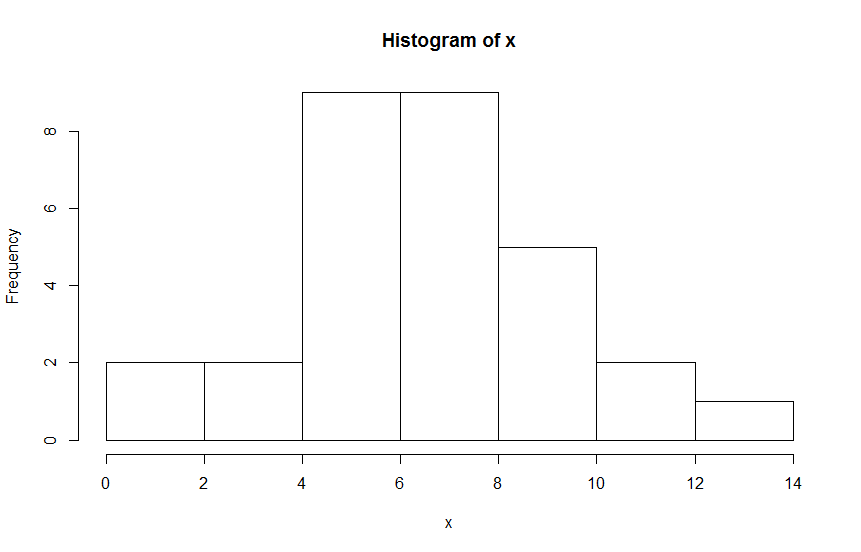
\includegraphics[scale=0.5]{Hist1.png}\\
\newpage
Задание 2\\
\begin{center}
 $Z = X\cdot sin(Y)$\\
 \end{center}
Составим ряд распределения случайной величины $Z$. Для этого для каждого $X$ подставим в формулу каждое значение $Y$, затем для полученных значений посчитаем вероятности, умножив соответствующую вероятность $X$ на вероятность $Y$. Получаем следующие таблицы.\\
\begin{lstlisting}[language=R,basicstyle=\normalsize]
x<-c(5,6,10,16,17)
y<-x
a<-matrix(0,5,5)
for(i in 1:length(x))
    for(j in 1:length(y))
        a[i,j]<-x[i]*sin(y[j])
print(a)
           [,1]      [,2]      [,3]      [,4]       [,5]
[1,]  -4.794621 -1.397077 -2.720106 -1.439517  -4.806987
[2,]  -5.753546 -1.676493 -3.264127 -1.727420  -5.768385
[3,]  -9.589243 -2.794155 -5.440211 -2.879033  -9.613975
[4,] -15.342788 -4.470648 -8.704338 -4.606453 -15.382360
[5,] -16.301713 -4.750063 -9.248359 -4.894356 -16.343757

px<-c(0.1553912,0.2683355,0.1841288,0.2818739,0.1102706)
py<-c(0.31514155,0.08008699,0.28486710,0.12811419,0.19179018)
b<-matrix(0,5,5)
for(i in 1:length(px))
    for(j in 1:length(py))
        b[i,j]<-px[i]*py[j]
print(b)
           [,1]       [,2]       [,3]       [,4]       [,5]
[1,] 0.04897022 0.01244481 0.04426584 0.01990782 0.02980251
[2,] 0.08456367 0.02149018 0.07643996 0.03437759 0.05146411
[3,] 0.05802664 0.01474632 0.05245224 0.02358951 0.03531410
[4,] 0.08883018 0.02257443 0.08029660 0.03611205 0.05406065
[5,] 0.03475085 0.00883124 0.03141247 0.01412723 0.02114882
\end{lstlisting}
Найдем математическое ожидание, дисперсию, стандартное отклонение и моду дискретной случайной величины Z:\\
$$M(Z)=\sum_{i=0}^{n}x_i p_i$$
$$D(Z)=M(Z^2)-(M(Z))^2$$
$$\sigma=\sqrt{D(Z)}$$\\
Модой случайной величины называется ее наиболее вероятное  значение. Для дискретной случайной величины - это значение, встречающееся с наибольшей частотой.По ряду распределения можно выявить, что модой случайной величины $Z$ является значение -15.342788.\\
\begin{lstlisting}[language=R,basicstyle=\normalsize]
Z<-c(-4.794621, -1.397077, -2.720106, -1.439517,  -4.806987,
     -5.753546, -1.676493, -3.264127, -1.727420,  -5.768385,
     -9.589243, -2.794155, -5.440211, -2.879033,  -9.613975,
     -15.342788, -4.470648, -8.704338, -4.606453, -15.382360,
     -16.301713, -4.750063, -9.248359, -4.894356, -16.343757)
P<-c(0.04897022, 0.01244481, 0.04426584, 0.01990782, 0.02980251,
     0.08456367, 0.02149018, 0.07643996, 0.03437759, 0.05146411,
     0.05802664, 0.01474632, 0.05245224, 0.02358951, 0.03531410,
     0.08883018, 0.02257443, 0.08029660, 0.03611205, 0.05406065,
     0.03475085, 0.00883124, 0.03141247, 0.01412723, 0.02114882)

m<-0
for(i in 1:length(Z))
    m<-Z[i]*P[i]+m
print(m)#M(Z)
[1] -7.437683
m2<-0
for(i in 1:length(Z))
    m2<-Z[i]*Z[i]*P[i]+m2
print(m2)#M(Z^2)
[1] 77.27161
d<-m2-m*m
print(d)#D(Z)
[1] 21.95249
sigma<-sqrt(d)
print(sigma)
[1] 4.685349
\end{lstlisting}
Запишем значения функции распределения в таблицу и построим ее график.\\ 
\begin{table}[!h]
\centering
%\caption{My caption}
\label{my-label}
\begin{tabular}{|l|l|l|}
\hline
\multicolumn{1}{|c|}{X\textless=0}         & F= & 0          \\ \hline
-16.343757\textless X\textless=-16.301713  & F= & 0.02114882 \\ \hline
-16.301713\textless X\textless=-15.382360  & F= & 0.05589967 \\ \hline
-15.382360\textless X\textless=-15.342788  & F= & 0.10996032 \\ \hline
-15.342788\textless X\textless=-9.613975   & F= & 0.1987905  \\ \hline
-9.613975\textless X\textless=-9.589243    & F= & 0.23411046 \\ \hline
-9.589243\textless X\textless=-9.248359    & F= & 0.29213134 \\ \hline
-9.248359\textless X\textless=-8.704338    & F= & 0.32354371 \\ \hline
-8.704338\textless X\textless=-5.768385    & F= & 0.40384031 \\ \hline
-5.768385\textless X\textless=-5.753546    & F= & 0.45530442 \\ \hline
-5.753546\textless X\textless=-5.440211    & F= & 0,53986809 \\ \hline
-5.440211\textless X\textless=-4.894356    & F= & 0.59232033 \\ \hline
-4.894356\textless X\textless=-4.806987    & F= & 0.60644756 \\ \hline
-4.806987\textless X\textless=-4.794621    & F= & 0.63625007 \\ \hline
-4.794621\textless X\textless=-4.750063    & F= & 0.68522029 \\ \hline
-4.750063\textless X\textless=-4.606453    & F= & 0.69405153 \\ \hline
-4.606453\textless X\textless=-4.470648    & F= & 0.73016358 \\ \hline
-4.470648\textless X\textless=-3.264127    & F= & 0.75273801 \\ \hline
-3.264127\textless X\textless=-2.879033    & F= & 0.82917797 \\ \hline
-2.879033\textless X\textless=-2.794155    & F= & 0.85276748 \\ \hline
-2.794155\textless X\textless=-2.720106    & F= & 0.8675138  \\ \hline
-2.720106\textless X\textless=-1.727420    & F= & 0.91177964 \\ \hline
-1.727420\textless X\textless=-1.676493    & F= & 0.94615723 \\ \hline
-1.676493\textless X\textless=-1.439517    & F= & 0.96764741 \\ \hline
-1.439517\textless X\textless=-1.397077    & F= & 0.98755523 \\ \hline
\multicolumn{1}{|c|}{-1.397077 < X} & F= & 1          \\ \hline
\end{tabular}
\end{table}
\newpage
\begin{figure}[!h]
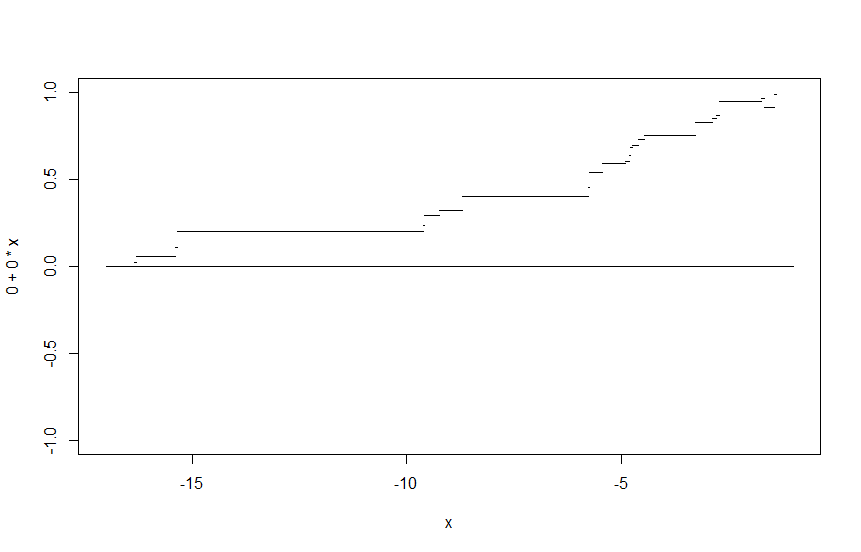
\includegraphics[scale=0.75,angle=90]{Rplot.png}\\
\end{figure}
